\documentclass{article}

\usepackage{times}
\usepackage{geometry}
\geometry{a4paper,left=0.6cm,right=0.7cm,top=1.5cm,bottom=1cm,columnsep=0.8cm}

\usepackage{fontawesome}          % icônes de base seulement
\usepackage[hidelinks]{hyperref}
\usepackage{multicol}
\usepackage{tikz}
\usepackage{hyphsubst}
\usepackage{moresize}
\usepackage{hyphenat}
\usepackage{tabularx}
\usepackage{xcolor}
\usepackage{enumitem}
\usetikzlibrary{calc, positioning}
\newcolumntype{Y}{>{\RaggedRight\arraybackslash}X}

% icônes manquantes -> puce
\makeatletter
\@for\sym:=faBrain,faMicrochip,faHandshakeO,faTools,faNetworkWired,%
             faDatabase,faServer,faGit,faUsers,faComments,faCalendar,faGroup\do{%
  \@ifundefined{\sym}{\expandafter\newcommand\csname\sym\endcsname{\textbullet}}{}}
\makeatother

% couleurs
\definecolor{maincolor}{HTML}{f0fafc}
\definecolor{seccolor}{HTML}{ffffff}
\definecolor{gray}{HTML}{8c94a9}
\definecolor{sidetext}{HTML}{59cee5}

% bande latérale bleue
\usepackage{eso-pic}
\AddToShipoutPictureBG{%
  \begin{tikzpicture}[remember picture,overlay]
    \fill[maincolor] (current page.north west) rectangle
                     ([xshift=0.3\paperwidth] current page.south west);
  \end{tikzpicture}%
}

% listes
\setlist[itemize]{itemsep=-2pt,topsep=0pt,leftmargin=1.08cm}
\renewcommand{\labelitemi}{\textcolor{sidetext}{\footnotesize$\bullet$}}

\setlength{\parindent}{0pt}
\usepackage{paracol}
\columnratio{0.3}

\begin{document}
\pagestyle{empty}

\begin{paracol}{2}
% ────────────────────────────────────────
% Colonne gauche
% ────────────────────────────────────────
\color{sidetext}
\vspace*{-0.5cm}

\noindent
\begin{minipage}{\linewidth}
  \centering
  \begin{tikzpicture}
    \clip (0,0) circle (1.5cm) node[anchor=center]
      {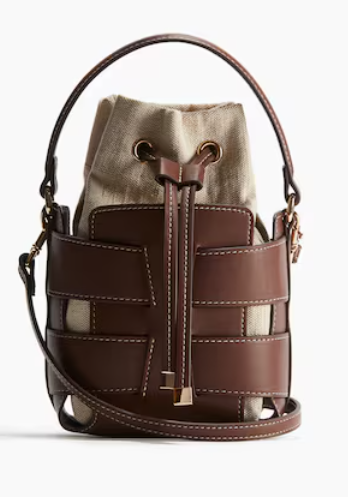
\includegraphics[width=3cm]{63c4e28752b84fd9b7618c1a96273185.png}};
  \end{tikzpicture}

  \vspace{3mm}
  {\color{black}\LARGE \textbf{Judikael Mourouvin}}

  \vspace{1mm}
  {\large Technicien informatique \& marketing digital}

  \vspace{3mm}
  {\color{gray}\rule{\linewidth}{0.4pt}} \\
\end{minipage}

% ── Coordonnées
\begin{tabular}{@{}c l}
  \faPhone &
  \begin{tabular}[t]{@{}l@{}}
    {\color{gray}Téléphone} \\ +590 690 91 14 48
  \end{tabular} \\
  \\
  \faLinkedin &
  \begin{tabular}[t]{@{}l@{}}
    {\color{gray}LinkedIn} \\
    \href{}{Mon LinkedIn}
  \end{tabular} \\
  \\
  \faMapMarker &
  \begin{tabular}[t]{@{}l@{}}
    {\color{gray}Adresse} \\ Route de COCOYER \\ 97190 Gosier
  \end{tabular} \\
  \\
  \faEnvelope &
  \begin{tabular}[t]{@{}l@{}}
    {\color{gray}Email} \\
    \href{mailto:jkmou971@gmail.com}{jkmou971@gmail.com}
  \end{tabular} \\
\end{tabular}

\vspace{2mm}
{\color{gray}\rule{\linewidth}{0.4pt}} \\

% ── Langues --------------------------------------------------------
{\color{black}{Langues}}

\vspace{2mm}
\begin{itemize}[leftmargin=*]
\item Anglais - \textcolor{gray}{}
\item Espagnol - \textcolor{gray}{}\end{itemize}          % ← le placeholder va contenir \begin{itemize}…\end{itemize}

{\color{gray}\rule{\linewidth}{0.4pt}} \\

% ── Compétences ----------------------------------------------------
\vspace{2mm}
{\color{black}{Compétences Clés}}

\vspace{2mm}
\begin{itemize}[leftmargin=*]
\item Réseaux
\item Maintenance
\item Support
\item Diagnostic
\item Marketing
\item Configuration
\item Administration\end{itemize}              % ← idem, une vraie liste
\vspace{2mm}
{\color{gray}\rule{\linewidth}{0.4pt}} \\

% ── Centres d'intérêt
\vspace{2mm}
{\color{black}{Centres d’intérêt}}

\vspace{2mm}
\begin{itemize}[leftmargin=*]
\item Lectur
\item Sports
\item Musique
\item Voyage
\end{itemize}     % ← simple itemize ou tabular

\vfill
~

% ────────────────────────────────────────
\switchcolumn
% Colonne droite
% ────────────────────────────────────────
\color{black}

% ── Profil
\textcolor{black}{\Large \textbf{Profil Professionnel}} \\[2pt]
Passionné par l'informatique et le marketing digital, j'ai développé des compétences solides en administration de systèmes, maintenance et support utilisateurs. Mon année d'alternance à la DSI de la Mairie du Gosier m'a permis de participer à des projets numériques et de contribuer à la stratégie digitale de l'organisation. Je souhaite désormais mettre mes connaissances techniques et mon sens du service au profit d'une nouvelle équipe à temps plein. Rigoureux, réactif et orienté résultats, je saurai accompagner vos utilisateurs et optimiser vos infrastructures. \\[8pt]

% ── Expérience
\textcolor{black}{\Large \textbf{Expérience Professionnelle}} \\[2pt]

\colorbox{maincolor}{%
  \begin{minipage}{\linewidth}
    \textbf{Alternant en Marketing Digital} \\ Mairie du Gosier, DSI \\ 2023-2024
    \begin{itemize}
      \item Géré des projets numériques municipaux, assurant le respect des délais et des exigences fonctionnelles \item Analysé les besoins des agents et déployé des solutions adaptées, améliorant leur productivité \item Assuré support et formations, renforçant l’autonomie des utilisateurs et la visibilité digitale de la collectivité
    \end{itemize}
  \end{minipage}}

\vspace{3mm}


\colorbox{maincolor}{%
  \begin{minipage}{\linewidth}
    \textbf{Animateur de la zone informatique} \\ Pôle Emploi, Gosier \\ 2022-2023
    \begin{itemize}
      \item Fourni assistance de proximité aux demandeurs et conseillers, réduisant les incidents récurrents \item Configuré et maintenu postes publics, garantissant leur disponibilité quotidienne \item Diagnostiqué et résolu pannes matérielles et logicielles, diminuant les temps d'arrêt
    \end{itemize}
  \end{minipage}}

\vspace{3mm}


\colorbox{maincolor}{%
  \begin{minipage}{\linewidth}
    \textbf{Stagiaire Informaticien} \\ Numerika, Baie-Mahault \\ 2020-2021
    \begin{itemize}
      \item Installé et entretenu équipements informatiques pour les clients, améliorant la fiabilité du parc \item Assuré support téléphonique et sur site, résolvant incidents de premier niveau \item Documenté procédures de maintenance, facilitant la prise en main par l'équipe
    \end{itemize}
  \end{minipage}}   % ← blocs \colorbox{maincolor}{\begin{minipage}…}

\vspace{8mm}

% ── Formation
\textcolor{black}{\Large \textbf{Formation}} \\[2pt]

    \begin{tabularx}{\linewidth}{@{}c >{\RaggedRight\arraybackslash}X@{}}
    \textcolor{sidetext}{\faGraduationCap} &
    \textbf{Bachelor Marketing Digital} \\
    & CFA IUTS \\
    & \textit{2023-2024} \\
    \end{tabularx}
    \begin{itemize}[leftmargin=*]
  \item Stratégie de communication et création de contenu numérique
  \item Gestion de projets web et analyse des performances marketing
  \item Outils d'acquisition de trafic et SEO/SEM
\end{itemize}
\vspace{3mm}

    \begin{tabularx}{\linewidth}{@{}c >{\RaggedRight\arraybackslash}X@{}}
    \textcolor{sidetext}{\faGraduationCap} &
    \textbf{BTS Système Numérique option Informatique et Réseaux} \\
    & Lycée de Chevalier Saint Georges, Abymes \\
    & \textit{2019-2021} \\
    \end{tabularx}
    \begin{itemize}[leftmargin=*]
  \item Architecture et administration de réseaux locaux
  \item Déploiement et maintenance de systèmes informatiques
  \item Support technique et notions de cybersécurité
\end{itemize}       % ← lignes tabular par diplôme

\end{paracol}
\end{document}

